% \begin{quotation}
% This program is free software: you can redistribute it and/or modify
% it under the terms of the GNU General Public License as published by
% the Free Software Foundation, either version 3 of the License, or
% (at your option) any later version.

% This program is distributed in the hope that it will be useful,
% but WITHOUT ANY WARRANTY; without even the implied warranty of
% MERCHANTABILITY or FITNESS FOR A PARTICULAR PURPOSE.  See the
% GNU General Public License for more details.

% You should have received a copy of the GNU General Public License
% along with this program.  If not, see <http://www.gnu.org/licenses/>.
% \end{quotation}

% Author: Chel Hee Lee
% Created on 2013-APR-11
% Modified on 2013-APR-11

% The HTML syntax generated from this document will be added to the page
% ./ihelp/www/sk_tips.html 
% htlatex $(file_name).tex "html, 4, mouseover, frames, next" "" "-dweb/"
% htlatex tips.tex "html, 1, mouseover, next"

% graphics file must be in the format of .eps


\documentclass{article}

\usepackage{mystyle}

\title{Some R Problems Derived Me Nuts Before!}
\author{iHELP Working Group \\ Chel Hee Lee \& Eugene Jung}

\begin{document}
\maketitle 

\paragraph{읽기전에:}
\texttt{R}을 사용하게 된 이래로 경험하게 된 여러가지 팁들을 정리한 것입니다.
% \textsf{본 페이지의 작성자는 다른 사용자들이 사용하는 놀라운 테크닉을 항상 배우고 있습니다}.
% 이 문서는 매일 하루에 하나의 팁이 올라올 수 있도록 노력할 예정입니다.

\paragraph{함께하는 방법:}
만약 이 페이지를 읽고 있는 독자님께서 가지고 계신 유용한 팁을 함께 공유하고자 하신다면, 그 내용을 \href{mailto:ihelp-urquestion@lists.r-forge.r-project.org}{ihelp-urquestion@lists.r-forge.r-project.org}로 보내주시길 부탁드립니다.
 
%%%%%%%%%%%%%%%%%%%%%%%%%%%%%%%%%%%%%%%%%%%%%%%%%%%%%%%%%%%%%%%%%%%%%%%%
%
% Data Management 
%
%%%%%%%%%%%%%%%%%%%%%%%%%%%%%%%%%%%%%%%%%%%%%%%%%%%%%%%%%%%%%%%%%%%%%%%%
\section{데이터 관리에 관련하여}

\begin{enumerate}
\item 결측치를 채우고 싶어요.

\item 여러개의 엑셀시트로 구성되어 있는 엑셀파일을 불러와 하나의 데이터셋으로 합치기 

\item 가끔 리스형으로 받아진 데이터가 중첩된 구조를 가지고 있어서, 한 번에 이를 불러오기를 해야할 때는 어떻게 해야할지.

\item \texttt{do.call()} 함수를 사용하는 법에 대해서..

\item 현재 패키지를 
\end{enumerate}

%%%%%%%%%%%%%%%%%%%%%%%%%%%%%%%%%%%%%%%%%%%%%%%%%%%%%%%%%%%%%%%%%%%%%%%%
%
% Numerical Techniques
%
%%%%%%%%%%%%%%%%%%%%%%%%%%%%%%%%%%%%%%%%%%%%%%%%%%%%%%%%%%%%%%%%%%%%%%%%

\section{수치해석 및 시뮬레이션에 관련하여}

\begin{enumerate}
\item \texttt{R}에도 \texttt{C}와 같은 \texttt{switch}문이 존재하나요?  -- 네 있습니다.

\item \texttt{warning}(경고)와 \texttt{error}(에러)를 이용하는 법

\item \texttt{try()} 함수를 이용하여 에러를 컨트롤 해보기 

\item \texttt{tryCatch()} 함수를 이용해서 에러를 컨트롤하기

\begin{Schunk}
\begin{Soutput}
result <- tryCatch(
{
	수행하고자 하는 표현식
}, 
warning = function(w) {
	위에서 수행한 표현식이 경고를 발생시킬때 어떻게 처리하고자 하는지에 대한 표현식
}, 
error = function(e) {
	위에서 수행한 표현식이 에러를 발생시킬때 어떻게 처리하고자 하는지에 대한 표현식 
}, finally {
	위에서 수행한 표현식에 대한 최종적 처리를 위한 표현식 
}
\end{Soutput}
\end{Schunk}

예제는 내일 시간날때 작성 
\item \texttt{combn()} 함수를 이용하여 모든 조합을 찾기 
\end{enumerate}



%%%%%%%%%%%%%%%%%%%%%%%%%%%%%%%%%%%%%%%%%%%%%%%%%%%%%%%%%%%%%%%%%%%%%%%%
%
% Visualization 
%
%%%%%%%%%%%%%%%%%%%%%%%%%%%%%%%%%%%%%%%%%%%%%%%%%%%%%%%%%%%%%%%%%%%%%%%%

\section{비쥬얼라이제이션}
\begin{enumerate}
\item \texttt{coordinating system}을 활용하기 

\item \texttt{Lattice} 패키지를 이용하여 아래와 같은 그림을 생성해보기 (가장 단순한 예제임 - 팁 보다는 튜토리얼 형식으로?)

%\rotatebox{-90}{\includegraphics{./lattice_ex1.eps}}
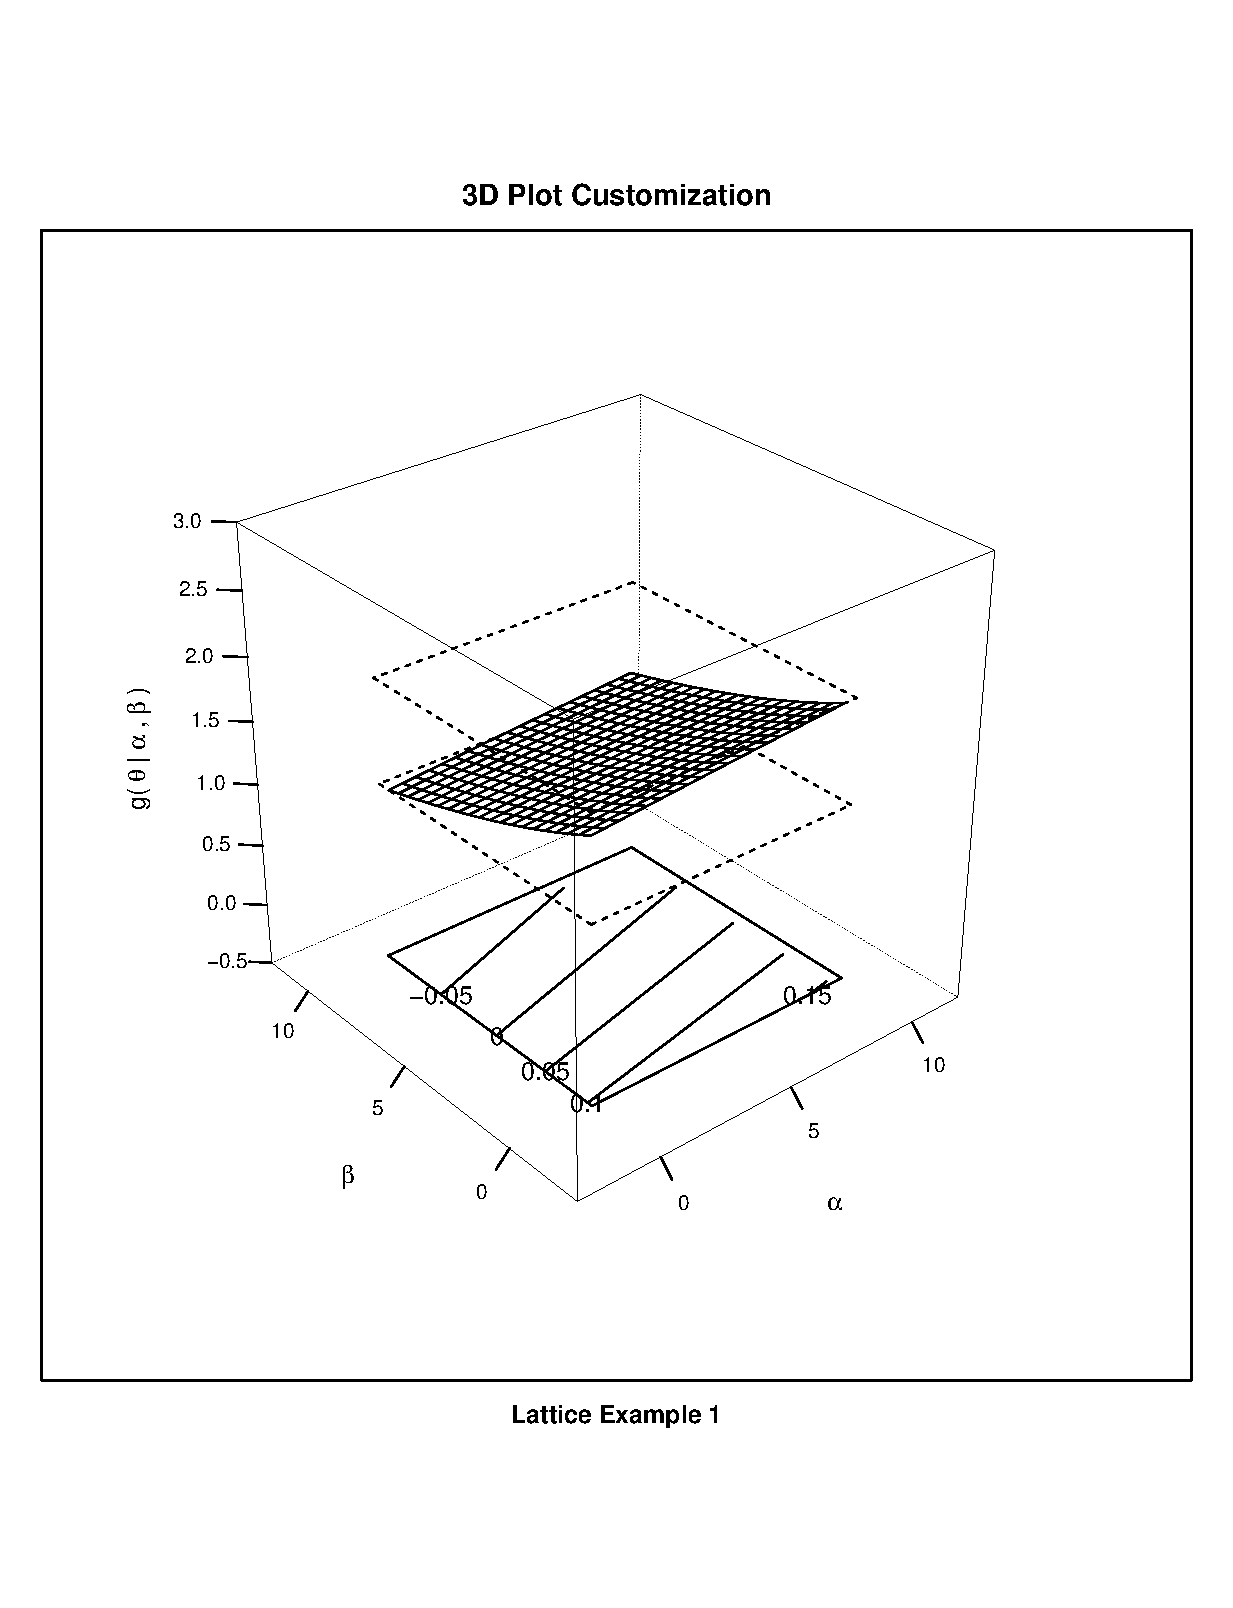
\includegraphics{./img/lattice-fig.eps}


\item \LaTeX 의 문서에 포함될 \texttt{.eps} 그래픽을 \texttt{R}에서 뽑았을 때는 아무런 문제가 없어 보였는데, 정작 \texttt{pdf}로 문서를 뽑아 보니까 이 그래픽이 들어간 페이지가 90도로 돌아가 있거나 혹은 그래픽이 90도로 회전되어 있을 경우에는 아래와 같이 하면 됩니다. 

\begin{Schunk}
 \begin{Sinput}
  postscript(file=``filename.eps'', onefile=FALSE, horizontal=FALSE)
 \end{Sinput}
\end{Schunk}

이 문제에 대한 출처는 \texttt{postscript} 도움말입니다. 

이문제를 다른 방법으로도 해결할 수 있습니다.  (대충 서너개 더 있음).
\end{enumerate}

%%%%%%%%%%%%%%%%%%%%%%%%%%%%%%%%%%%%%%%%%%%%%%%%%%%%%%%%%%%%%%%%%%%%%%%%
%
% Utilities
%
%%%%%%%%%%%%%%%%%%%%%%%%%%%%%%%%%%%%%%%%%%%%%%%%%%%%%%%%%%%%%%%%%%%%%%%%

\section{데이터 입출력 및 파일관리 유틸리티}
\begin{enumerate}
\item \texttt{read.table} 계열의 함수를 이용하여 데이터를 불러올 때 첫번째 인자는 파일의 위치와 파일명이 입력된 문자열이어야 합니다.
그런데, 간혹 문법에서 틀린 점도 없고, 불러오고자 하는 데이터 파일도 올바른 파일경로에 위치하고 있음에도 불구하고,
데이터를 찾을 수 없다고 하는 경우가 있습니다. 
이것은 내부적으로 파일경로에 띄어쓰기, 특수문자, 혹은 특수한 인코딩 등 다양한 이유로 인하여 파일경로가 올바르게 처리되지 않았기 때문입니다.
아래와 같은 방법으로 \texttt{read.table()} 함수 사용시 \texttt{file.choose()} 함수를 함께 사용하면 이러한 문제를 해결이 가능합니다.


\begin{Schunk}
\begin{Soutput}
mydata <- read.table(file.choose(), header=TRUE, sep=",")
\end{Soutput}
\end{Schunk}


\end{enumerate}


%%%%%%%%%%%%%%%%%%%%%%%%%%%%%%%%%%%%%%%%%%%%%%%%%%%%%%%%%%%%%%%%%%%%%%%%
%
% Miscellinous
%
%%%%%%%%%%%%%%%%%%%%%%%%%%%%%%%%%%%%%%%%%%%%%%%%%%%%%%%%%%%%%%%%%%%%%%%%

\section{기타내용들}
\begin{enumerate}
\item 불러오고자 하는 데이터의 인코딩이 UTF-8가 아닐때 이를 확인하고, 데이터를 올바르게 불러오기 위한 내용은 \url{http://lists.r-forge.r-project.org/pipermail/ihelp-urquestion/2013-April/000017.html}를 읽어보시길 바랍니다. 

\item \texttt{R}을 한국어가 아닌 영문으로 사용하고 싶습니다 (버전에 관계없이 일반적으로 통용되는 방법 - 윈도우즈 사용자에게 맞추어 작성됨).
이를 설정하는 방법에 대해서는 \url{http://lists.r-forge.r-project.org/pipermail/ihelp-urquestion/2013-April/000003.html}을 읽어보시길 바랍니다. 
\end{enumerate}

\end{document}
